\documentclass[tikz,border=8pt]{standalone}
\usepackage[T1]{fontenc}
\usepackage{helvet}
\renewcommand{\familydefault}{\sfdefault}
\usetikzlibrary{arrows.meta}

\definecolor{queryfill}{HTML}{DFF7F3}
\definecolor{queryborder}{HTML}{1BA99C}
\definecolor{corpusfill}{HTML}{FFF4D6}
\definecolor{corpusborder}{HTML}{D9A441}
\definecolor{llmfill}{HTML}{E9EDFF}
\definecolor{llmborder}{HTML}{6979C9}
\definecolor{nodefill}{HTML}{E8F2FF}
\definecolor{nodeborder}{HTML}{4E8CD8}
\definecolor{outfill}{HTML}{E7F6E7}
\definecolor{outborder}{HTML}{4FA64F}
\definecolor{softgray}{HTML}{F4F7FB}
\definecolor{darkline}{HTML}{333333}

\tikzset{
  card/.style={rectangle, rounded corners=5pt, align=center, draw=darkline, line width=0.8pt, minimum height=0.82cm, font=\small},
  query/.style={card, fill=queryfill, draw=queryborder, minimum width=2.05cm},
  corpus/.style={card, fill=corpusfill, draw=corpusborder, minimum width=2.25cm},
  llm/.style={card, fill=llmfill, draw=llmborder, minimum width=2.75cm, font=\small\bfseries},
  artifact/.style={card, fill=white, minimum width=2.75cm},
  output/.style={card, fill=outfill, draw=outborder, minimum width=2.75cm},
  softbox/.style={rectangle, rounded corners=8pt, draw=darkline, fill=softgray, line width=0.7pt},
  doc/.style={rectangle, rounded corners=4pt, fill=corpusfill, draw=corpusborder, line width=0.7pt, minimum width=0.42cm, minimum height=0.58cm},
  node/.style={circle, fill=nodefill, draw=nodeborder, line width=0.7pt, minimum size=0.29cm},
  finalnode/.style={circle, fill=outfill, draw=outborder, line width=0.7pt, minimum size=0.29cm},
  phase/.style={font=\small\bfseries, align=center},
  flow/.style={-{Latex[length=2.2mm]}, line width=0.85pt, draw=darkline},
  faint/.style={dashed, darkline, opacity=0.32}
}

\begin{document}
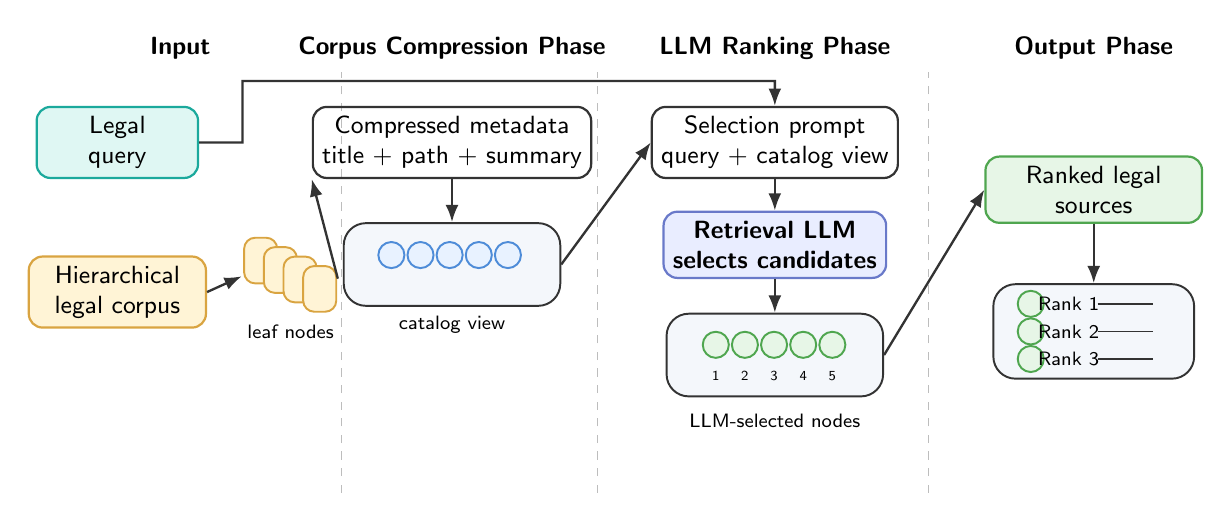
\begin{tikzpicture}

\node[phase] at (1.1,5.65) {Input};
\node[phase] at (4.55,5.65) {Corpus Compression Phase};
\node[phase] at (8.65,5.65) {LLM Ranking Phase};
\node[phase] at (12.7,5.65) {Output Phase};

\node[query] (query) at (0.3,4.45) {Legal\\query};
\node[corpus] (corpus) at (0.3,2.55) {Hierarchical\\legal corpus};

\foreach \x/\y in {2.12/2.95,2.37/2.83,2.62/2.71,2.87/2.59} {
  \node[doc] at (\x,\y) {};
}
\node[font=\scriptsize] at (2.5,2.04) {leaf nodes};

\node[artifact] (metadata) at (4.55,4.45) {Compressed metadata\\title + path + summary};
\node[softbox, minimum width=2.75cm, minimum height=1.05cm] (catalog) at (4.55,2.9) {};
\foreach \x in {3.78,4.15,4.52,4.89,5.26} {
  \node[node] at (\x,3.02) {};
}
\node[font=\scriptsize] at (4.55,2.14) {catalog view};

\node[artifact] (prompt) at (8.65,4.45) {Selection prompt\\query + catalog view};
\node[llm] (select) at (8.65,3.15) {Retrieval LLM\\selects candidates};
\node[softbox, minimum width=2.75cm, minimum height=1.05cm] (survivors) at (8.65,1.75) {};
\foreach \x/\lab in {7.9/1,8.27/2,8.64/3,9.01/4,9.38/5} {
  \node[finalnode] at (\x,1.88) {};
  \node[font=\tiny] at (\x,1.48) {\lab};
}
\node[font=\scriptsize] at (8.65,0.92) {LLM-selected nodes};

\node[output] (sources) at (12.7,3.85) {Ranked legal\\sources};
\node[softbox, minimum width=2.55cm, minimum height=1.2cm] (rankbox) at (12.7,2.05) {};
\foreach \y/\lab in {2.4/1,2.05/2,1.7/3} {
  \node[finalnode] at (11.9,\y) {};
  \node[font=\scriptsize] at (12.38,\y) {Rank \lab};
  \draw[darkline, line width=0.5pt] (12.75,\y) -- (13.45,\y);
}

\draw[flow] (query.east) -- ++(0.55,0) -- ++(0,0.78) -- (8.65,5.23) -- (prompt.north);
\draw[flow] (corpus.east) -- (1.88,2.75);
\draw[flow] (3.1,2.72) -- (metadata.south west);
\draw[flow] (metadata) -- (catalog);
\draw[flow] (catalog.east) -- (prompt.west);
\draw[flow] (prompt) -- (select);
\draw[flow] (select) -- (survivors);
\draw[flow] (survivors.east) -- (sources.west);
\draw[flow] (sources) -- (rankbox);

\draw[faint] (3.15,0.0) -- (3.15,5.35);
\draw[faint] (6.4,0.0) -- (6.4,5.35);
\draw[faint] (10.6,0.0) -- (10.6,5.35);

\end{tikzpicture}
\end{document}
